% !TEX root =  ../ReplyLetterMain.tex
\clearpage
\section*{Response to 1st Referee's Comments}
We would like to thank the Referee for his/her constructive comments, which have allowed us to considerably improve our paper. The main differences of the new version of the manuscript compared to the previous one can be found in Sections~5 and 6, Web Appendix A.2, C and D. In addition, changes regarding the specific comments have been made throughout the text.

You may find below our responses to the specific issues raised.

\begin{enumerate}

	\item 
	\underline{Assumption of normality of random effects and error term.}

	We thank the Referee for motivating us to check these assumptions in detail. We found that our model did not satisfy the assumptions of normality of error terms. To this end, we discuss our solution for this issue in the following paragraph. The issue of assumption of normality of random effects is discussed in the last paragraph.

	With regards to the assumption of normality of error term, we used residual diagnostics to check this assumption. The left panel of Figure \ref{fig : qqplot_norm_t3} shows the quantile-quantile (q-q) plot of subject specific residuals under our original joint model (JM). This figure suggests that a symmetric long tailed distribution for errors is more plausible than the normal distribution. Based on this result, we further fitted two JMs with t-distributed errors, with 4 and 3 degrees of freedom (df), respectively. We found that the model with t-distributed (df=3) errors satisfied the distributional assumptions the best (see Figure \ref{fig : qqplot_norm_t3}). 

	\begin{figure}[!htb]
	\centerline{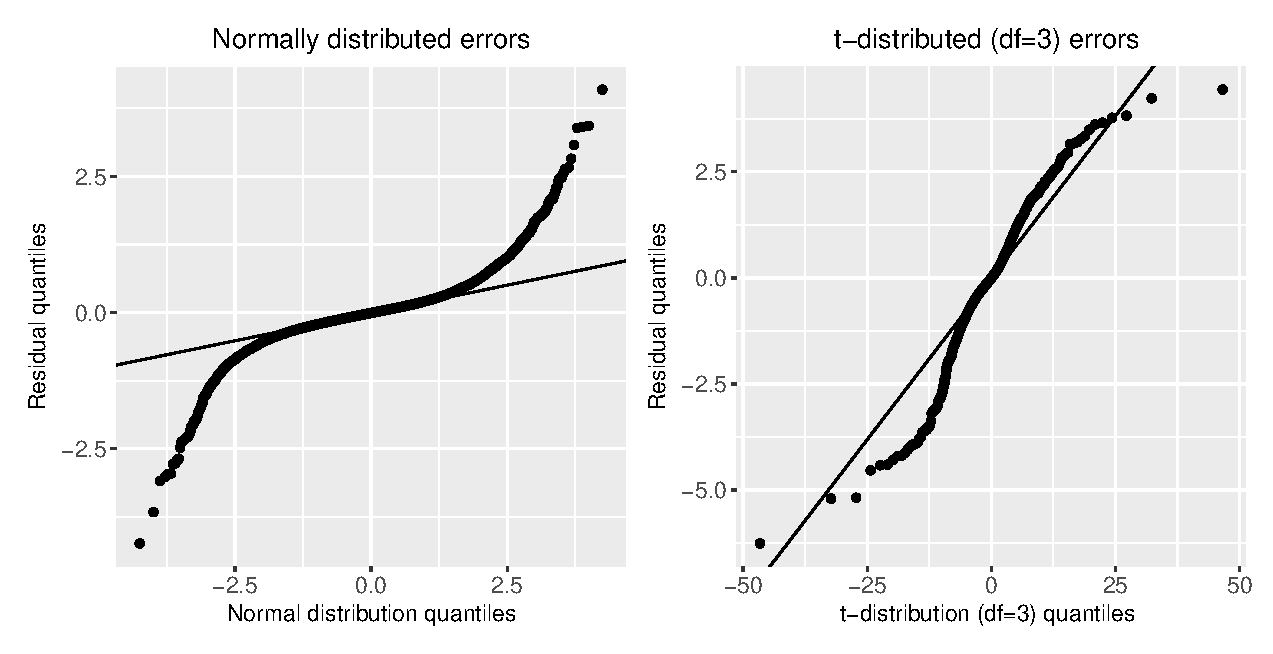
\includegraphics[width=\columnwidth]{images/model_fit/qqplot_norm_t3.eps}}
	\caption{Quantile-quantile plots of subject specific residuals obtained from the joint models with assumption of normally distributed errors, and t-distributed (df=3) errors, fitted to the PRIAS data set.}
	\label{fig : qqplot_norm_t3}
	\end{figure}

	We then compared the model with the assumption that errors are normally distributed and the model with assumption that errors are t-distributed. To this end, the fitted marginal $\log_2 \mbox{PSA}$ profile for a hypothetical patient with age 70 years using the two models is shown in Figure \ref{fig : marginal_fitted_psa_NormalVsT3}. We also compared the subject specific fitted $\log_2 \mbox{PSA}$ profiles for 9 randomly selected patients (each with more than 3 observations). Lastly, for the two models, Table \ref{tab : relative_risk_comparison} shows the association parameters. We can see that the association between the hazard of GR and slope of $\log_2 \mbox{PSA}$ is stronger in the model with t-distributed (df=3) errors. We have updated the parameter estimates for the new JM in \ref{sec : param_estimates_jm_fit_prias} of the revised supplementary material.

	\begin{table}[!htb]
	\begin{center}
	\caption{Relative risk sub-model estimates for association parameters between hazard of GR and slope of $\log_2 \mbox{PSA}$ levels. Mean and 95\% credible interval (CI) are presented for fits obtained from the joint models with assumption of normal distributed errors, and t-distributed (df=3) errors.}
	\label{tab : relative_risk_comparison}
	\begin{tabular}{lrr}
	\Hline
	Error distribution                      & $\log_2 \mbox{PSA}$ association [95\% CI]   & Slope($\log_2 \mbox{PSA}$) association [95\% CI]\\ 
	\hline
	t-distribution (df=3)                  & -0.004 [-0.119, 0.117] & 2.888 [2.318, 3.452] \\
	Normal distribution                    & -0.049 [-0.172, 0.078] & 2.407 [1.791, 3.069] \\
	\hline
	\end{tabular}	
	\end{center}
	\end{table}

	\begin{figure}[!htb]
	\centerline{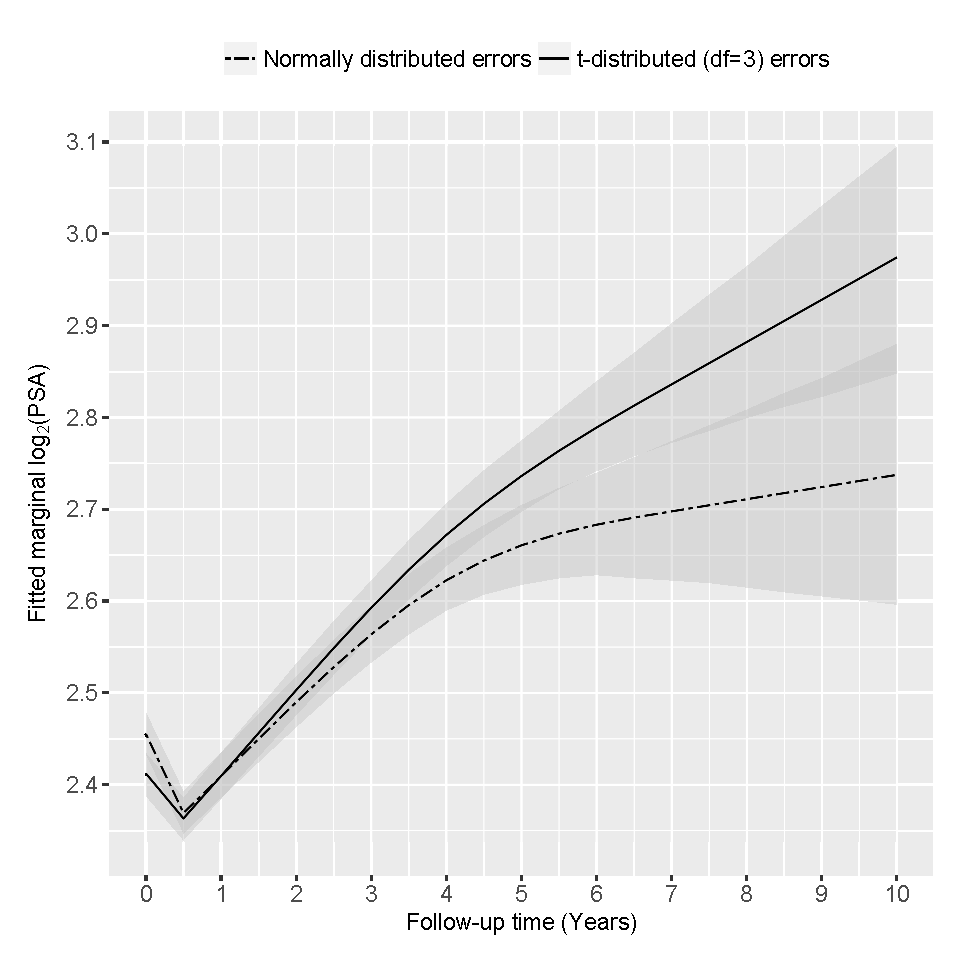
\includegraphics[width=0.75\columnwidth]{images/model_fit/marginal_fitted_psa_NormalVsT3.eps}}
	\caption{Fitted marginal 10 year $\log_2 \mbox{PSA}$ profile with 95\% credible interval (CI), for a hypothetical patient who was included in AS at the age of 70 years. Fits were obtained from joint models with assumption of normal distributed errors, and t-distributed (df=3) errors. The darker shaded region indicates the overlap in the two CI intervals, as well as demarcates the two sets of CIs.}
	\label{fig : marginal_fitted_psa_NormalVsT3}
	\end{figure}		
	
    \begin{figure}[!htb]
	\centerline{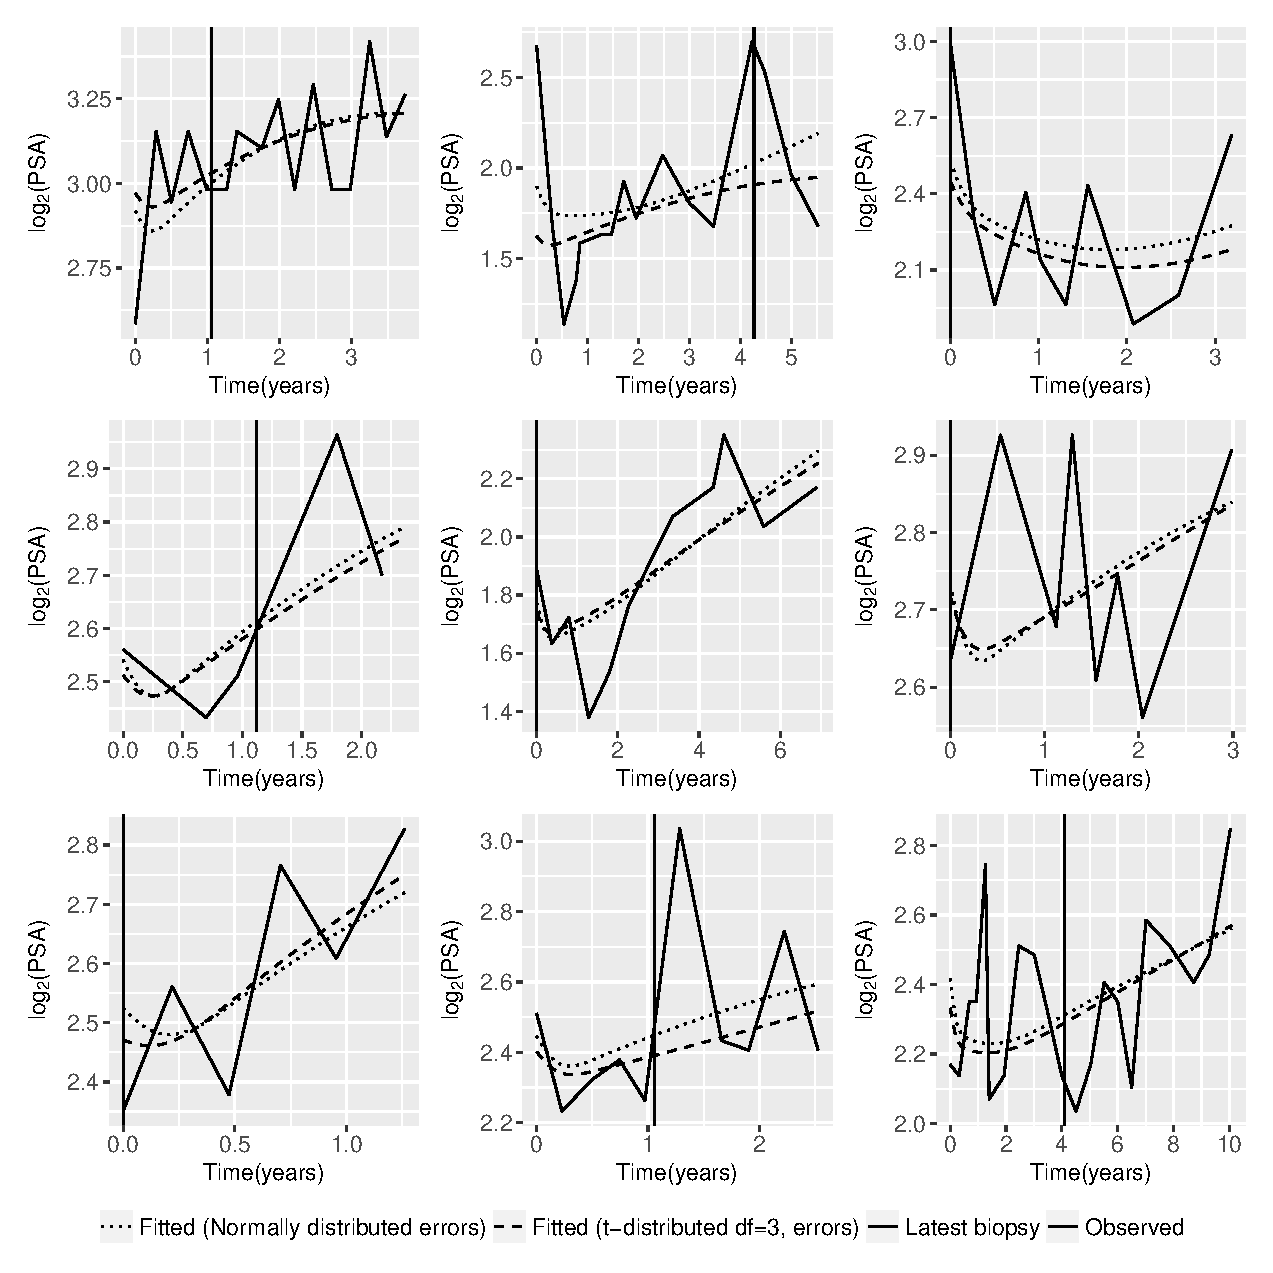
\includegraphics[width=\columnwidth]{images/model_fit/subject_fittedVsObserved_psa_norm_t3.eps}}
	\caption{Fitted versus observed $\log_2 \mbox{PSA}$ profiles for 9 randomly selected patients. Fits were obtained from joint models with assumption of normal distributed errors, and t-distributed (df=3) errors. The fitted profiles utilize information from both the observed PSA levels and time of latest biopsy.}
	\label{fig : subject_fittedVsObserved_psa_norm_t3}
	\end{figure}

	Since the slope association between $\log_2 \mbox{PSA}$ levels and hazard of Gleason reclassification (GR) in the model with t-distributed (df=3) errors, has become stronger, we expect our schedules to become slightly more sensitive towards increase in $\log_2 \mbox{PSA}$ velocity. This however, also depends on the type of personalized schedule. For example, we compared the personalized schedule based on dynamic risk of GR using the two different models for the three demonstration patients, and observed trivial differences. This is due to the fact that average risk (averaged over all time points) taken by dynamic risk of GR is not very high (5.3\%). However quantiles corresponding to 50\% risk (median time of GR) may differ by a bigger margin depending upon the profile of the patient (same for expected failure time). We next discuss the impact of the new association parameter on the schedules for the three patients.

	We can see in Figure \ref{fig : demo_expfail_norm_t3} (bottom row) and Figure \ref{fig : variance_demo_patients_norm_t3} that the third demonstration patient has a consistent profile, with a quite slow rise in PSA. Consequently the effect of the increased $\log_2 \mbox{PSA}$ slope association parameter does not affect the schedule much for this patient. Similar results are observed for the first demonstration patient when the PSA consistently remains low over nearly three years, starting at year two (Figure \ref{fig : demo_expfail_norm_t3}, top row, rightmost panel). Lastly, this can also be seen for the second demonstration patient wherein the schedules differ by a large margin initially when the PSA rises very quickly. However the gap becomes slightly smaller after a negative biopsy indicating that GR is unlikely in near future. Thus we expect that the sensitivity of the schedule based on expected failure time is within acceptable boundaries for slowly progressing (low risk) patients with consistent profiles.

	\begin{figure}[!htb]
	\centerline{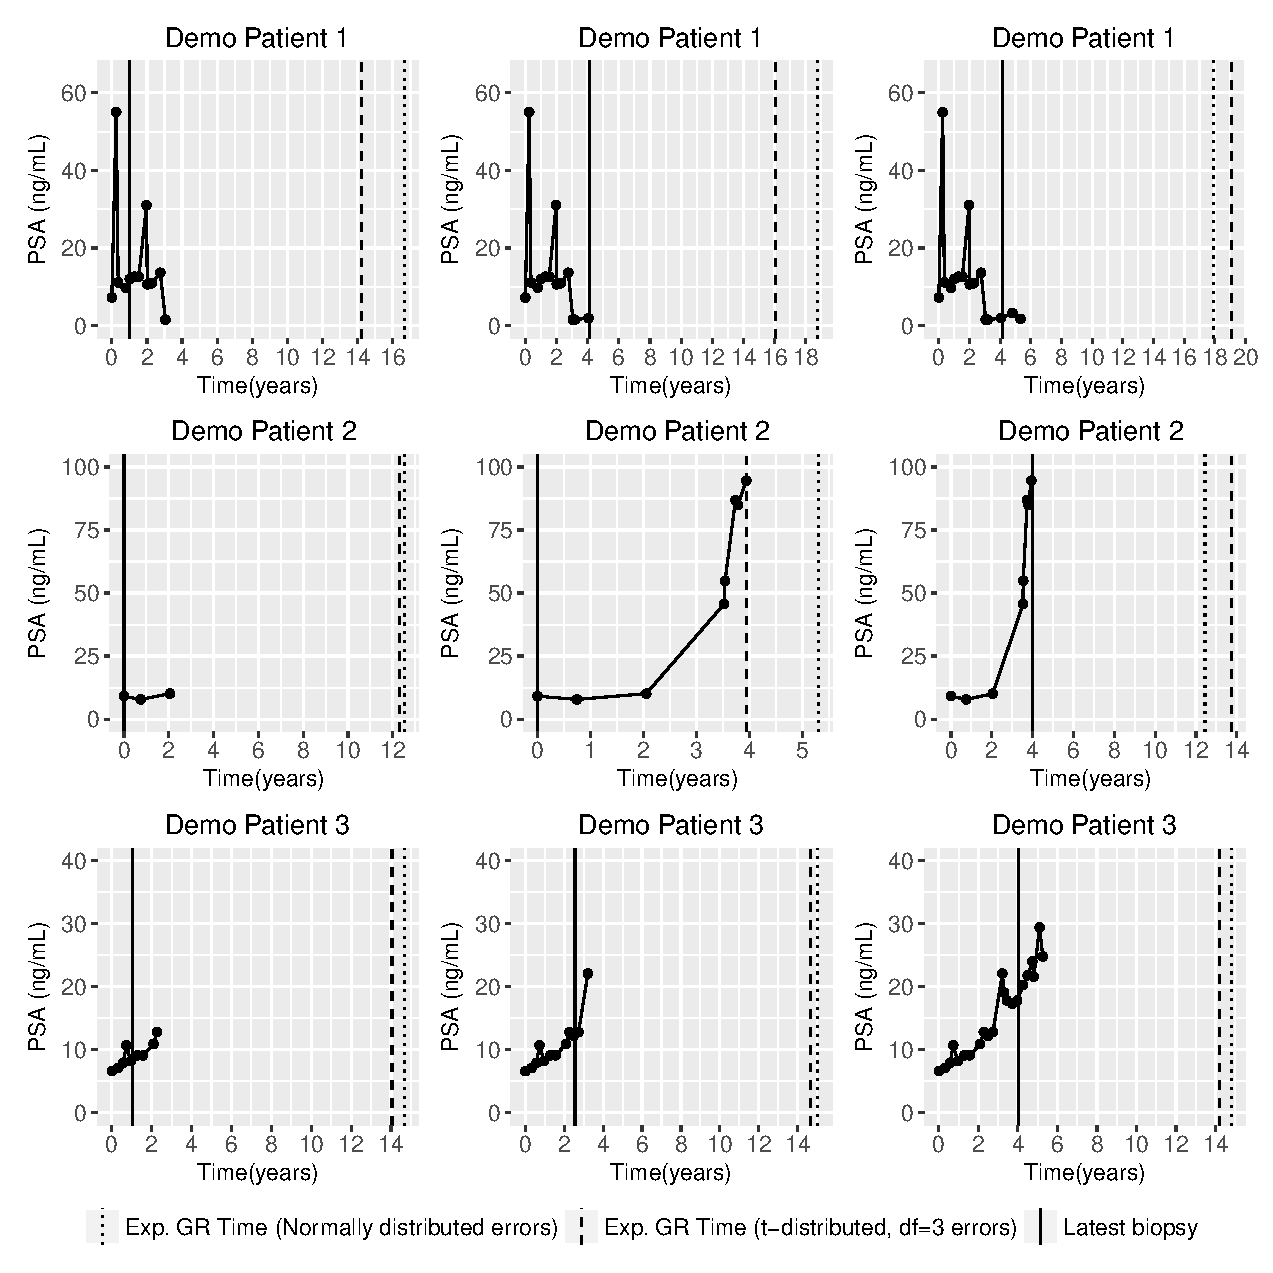
\includegraphics[width=\columnwidth]{images/model_fit/demo_expfail_norm_t3.eps}}
	\caption{Dynamic expected failure time for the three demonstration patients at three different follow-up times, using joint models with assumption of normal distributed errors, and t-distributed (df=3) errors.}
	\label{fig : demo_expfail_norm_t3}
	\end{figure}

	\begin{figure}[!htb]
	\centerline{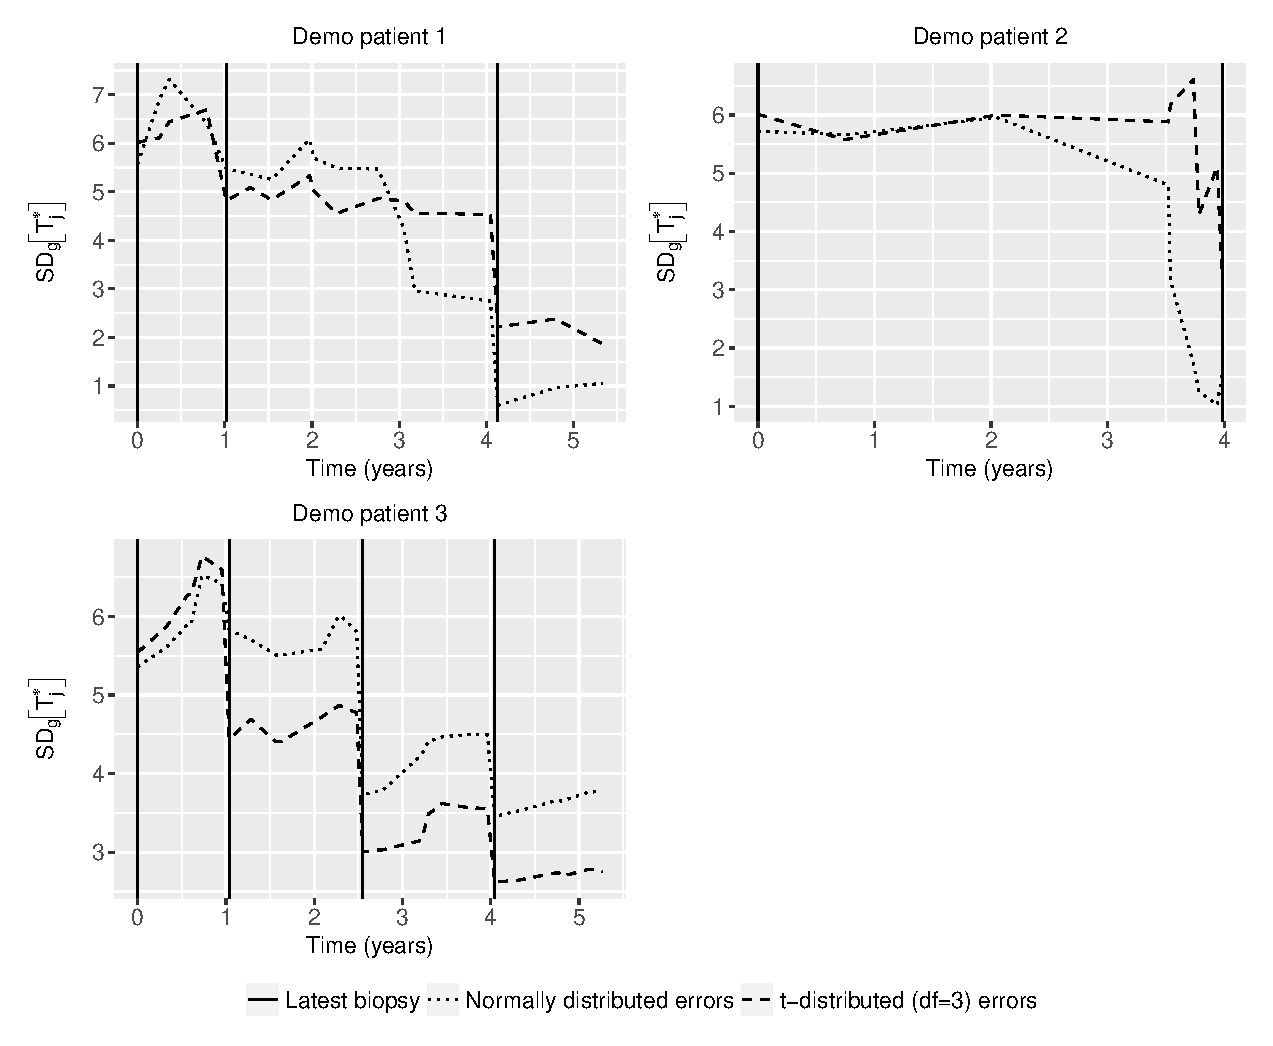
\includegraphics[width=\columnwidth]{images/model_fit/variance_demo_patients_norm_t3.eps}}
	\caption{Dynamic variance of the posterior predictive distribution of event time for the three demonstration patients at three different follow-up times, using joint models with assumption of normal distributed errors, and t-distributed (df=3) errors.}
	\label{fig : variance_demo_patients_norm_t3}
	\end{figure}

	With regards assumption of normality of random effects, JMs have been shown to be quite robust to random effects misspecification. More specifically, \citet*{rizopoulos2008shared,huang2009latent} have shown that unless the number of repeated measurements per patient are extremely small, such misspecification only and trivially affects the standard errors. In our dataset we have a mean of 8.7 measurements per patient, which makes us feel confident with regards to this assumption.

	\item \underline{Choice of demonstration patients, and cross validation using PRIAS dataset.}

	The three demonstration patients were chosen on the basis of specific characteristics of their data. This is because we wanted to demonstrate three main features of the personalized schedules. In particular, the first demonstration patient had many repeat biopsies, and thus via his profile we show how the variance of posterior predictive distribution of GR time decreases with each biopsy. Via the second demonstration patient we show how the schedules change with changes in PSA alone (no repeat biopsies). Whereas, via the third demonstration patient we show how the schedules work when information from PSA and repeat biopsies is not in concordance with each other.

	With regards to conducting cross-validation on real data, and to compare the true GR time of PRIAS patients who obtained GR, with the time proposed by personalized schedules, this is not possible for the following reason. For patients in PRIAS if our method proposes a time $u$ of the biopsy, we cannot conduct it at time $u$ because biopsies are already conducted for the patients as per PRIAS schedule. Secondly, we only know the interval $l_i < T^*_i \leq r_i$ in which GR occurred and not the true GR time $T^*_i$. On top of that this is known only for 707 out of 5267 patients, and the rest are right censored. That is, in either case we cannot calculate the offset $T^S_i - T^*_i$ of our schedule, where $T^S_i > T^*_i$ is the time of the last biopsy at which GR is detected. In this regard, the simulation study is our attempt to objectively evaluate our proposed method versus the fixed-schedule approach.

	\item \underline{Stratified relative risk model for modeling baseline hazards in simulation study.}

	We would like to thank the Reviewer for raising this point. Indeed in our simulation study we have assumed that there are three equal sized subgroups $G_1$, $G_2$ and $G_3$ of patients in the population, differing in the baseline hazard of GR. This was done because we wanted to test the performance of different schedules for a population with a mixture of patients, namely those with faster progressing PCa, as well as those with slowly progressing PCa. As correctly advised by the Referee these can be modeled using a stratified modeling approach. In the current case, this corresponds to the use of latent class JMs \citep{proust2014joint}. Even though our approach could also be formulated under the latent class model, this extension falls outside the scope of our paper that primarily aims introducing our proposed procedure for personalized scheduling of biopsies. Moreover, we expect that our postulated penalized B-spline approximation of the log baseline hazard (see \ref{web_sec : jm_framework}) captures the assumed mixture of Weibull hazards adequately. Figure \ref{fig : fitted_baseline_hazard} shows a comparison between the fitted and theoretical hazard. We observe that the fit of the B-spline is close to the theoretical baseline hazard.

	\begin{figure}[!htb]
	\centerline{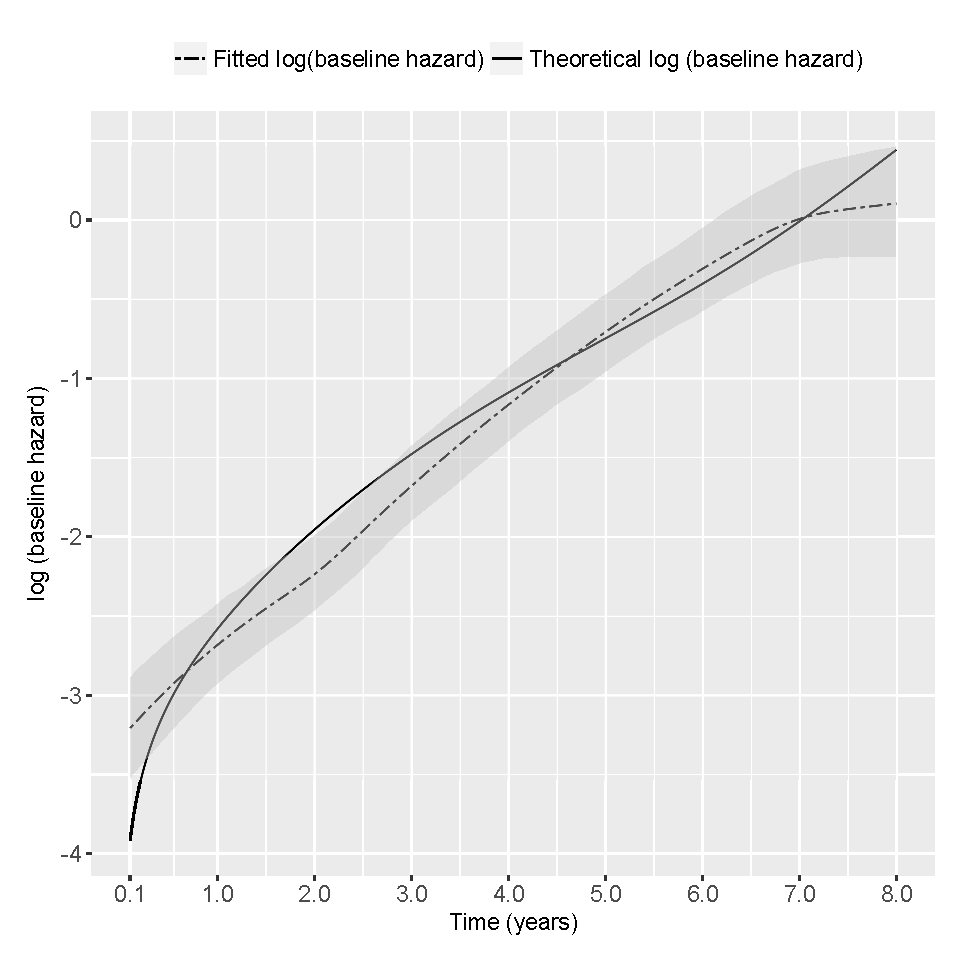
\includegraphics[width=0.75\columnwidth]{images/sim_study/baseline_hazard.eps}}
	\caption{Theoretical log baseline hazard of the simulated population versus mean of the fitted log baseline hazard. The 95\% confidence interval for the fitted log baseline hazard is obtained from the 500 simulations.}
	\label{fig : fitted_baseline_hazard}
	\end{figure}

	\item \underline{Bias due to biopsy schedule depending upon PSA-DT.}

	The Reviewer raises an important point. Indeed PRIAS switches to the more frequent annual schedule if a patient's PSA doubling time (PSA-DT), measured as the inverse of the slope of the regression line through the base two logarithm of PSA values, is less than 10 years. This raises the concern of (ascertainment) bias caused by the fact that the schedule of biopsies depends on past PSA levels. 
	Nevertheless, working under the framework of JMs has the advantageous feature that we can ignore the PSA-DT process and obtain valid parameter estimates, under the condition that the model is correctly specified. This is due to the fact that the joint model uses a full likelihood specification for the longitudinal and event time processes \citep{tsiatis2004joint}. To show this, consider the following full general specification of the JM that we use. Let $\boldsymbol{y}_i$ denote the $n_i \times 1$ vector of PSA measurements for the $i$-th patient, and $l_i, r_i$ denote the two time points of the interval in which GR occurs for the $i$-th patient. In addition let $T_i^S$ and $\mathcal{V}_i$ denote the schedule of biopsies and schedule of PSA measurements, respectively. Under the assumption that both of these schedules may depend upon only the observed $\boldsymbol{y}_i$, the joint likelihood of all four processes is given by:

	\begin{equation}
	\label{eq : decomposition_likelihood}
	p(\boldsymbol{y}_i, l_i, r_i, T_i^S, \mathcal{V}_i \mid \boldsymbol{\theta}, \boldsymbol{\psi}) = p(\boldsymbol{y}_i, l_i, r_i \mid \theta) \times p(T_i^S, \mathcal{V}_i \mid \boldsymbol{y}_i, \boldsymbol{\psi}).
	\end{equation}

	From this decomposition we can see that even if the processes $T_i^S$ and $\mathcal{V}_i$ may be determined from $\boldsymbol{y}_i$, if we are interested in the parameters $\boldsymbol{\theta}$ of the joint distribution of longitudinal and event outcome, the second term only contributes a constant in the likelihood and hence can be ignored. To check if we correctly specified the JM, we performed several sensitivity analysis in our model (e.g., changing the position of the knots, etc.) to investigate the fit of the model and also the robustness of the results. In all of our attempts, the same conclusions were reached, namely that the $\log_2 \mbox{PSA}$ velocity is more strongly associated with the hazard of GR compared to the $\log_2 \mbox{PSA}$ levels.

	The Referee has also asked an interesting question about the use of right censored data in the simulation study instead of interval censored data, given that the PRIAS data is also interval censored. However, in the simulation study even if we would have generated interval censored data it would not have led to any nontrivial differences in results. The reason is that we use a full likelihood approach as described in Section \ref{sec : jm_framework} of the original manuscript. Parameter estimation using full likelihood approaches always gives consistent and asymptotically unbiased results \citep{gentleman1994maximum}, under the condition that the model is correctly specified. In the current context, we correctly use an interval censoring specification of the joint likelihood when the data is interval censored, and right censoring specification when the (simulated) data is right censored.

	\item \underline{AUC comparison for JM with value and velocity association, and only value association.}
	
	We thank the Referee for noticing the erroneous result that was reported. The two sets of AUC's were mistakenly swapped while creating \ref{tab : AUC} in the original supplementary material, and hence the counterintuitive results. We have corrected this mistake, and in addition as advised by the Referee, we have also reported the confidence interval. The resulting estimates are presented in Table \ref{tab : AUC_reply_letter} below, as well as added in Supplementary material (\ref{tab : AUC}).

	\begin{table}[!htb]
	\begin{center}
	\caption{Area under the receiver operating characteristic curves, and 95\% confidence interval in brackets.}
	\label{tab : AUC_reply_letter}
	\begin{tabular}{rrr}
\Hline
Year                      & $\log_2 \mbox{PSA}$ value and velocity association & $\log_2 \mbox{PSA}$ value association\\ 
\hline
1 & 0.613 [0.582, 0.632] & 0.595 [0.565, 0.618]\\
2 & 0.648 [0.608, 0.685] & 0.609 [0.568, 0.654]\\
3 & 0.593 [0.560, 0.638] & 0.590 [0.536, 0.628]\\
\hline
	\end{tabular}	
	\end{center}
	\end{table}

	\item \underline{Typographic errors in equations.}
	
	We thank the Referee for pointing out these errors. We have corrected these in the revised version of the manuscript.

\end{enumerate}

